\section{Empirical Results}
In this section, we will show our empirical results about the relation between BLEU with Semantic Score. We use Pearson\rq s correlation coefficient \cite{PearsonCorrelation}to gauge how strong their relationship. The correlation coefficient has value between -1 and 1, where 1 indicates a strong positive relationship, -1 indicates a strong negative relationship, and 0 indicates no relationship at all. 

Figures \ref{fig:BleuSemlpSMT}, \ref{fig:BleuSemMppSMT}  show the scatter plots between 2 metrics: BLEU and Semantic. Each point represents scores of a pair of methods where its x-axis value is BLEU score and y-axis value is Semantic score.
The correlation coefficient between BLEU and Semantic score for the model mppSMT is 0.524 and for the model lpSMT is 0.62. That meant there is a positive relationship between the two metrics, but it is not strong since the correlation is closer to 0.5 than to 1.0. The two figures \ref{fig:BleuSemlpSMT} and \ref{fig:BleuSemMppSMT} also demonstrate the weak correlation on the following observations:  

\emph{Observation 1:} For a fixed value of Semantic score, there can be many associated BLEU values. Specifically, in the model lpSMT, with a Semantic Score of 1, the BLEU scores can be varied greatly between 0-1, which was reflected on the top horizontal line of dots in figure \ref{fig:BleuSemlpSMT}. Similarly, in the figure \ref{fig:BleuSemMppSMT}, with a Semantic Score of 1, the BLEU scores are in the range of 0.5 to 1. 

\emph{Observation 2:} For a fixed value of BLEU, there can be many associated Semantic scores. For an instance, the figure \ref{fig:BleuSemMppSMT} shows that for a high BLEU score, for example value around 0.75, can have Semantic Score from 0.25 to 1. This can be observed by the vertical line of dots in the figure. 

\emph{Implication 1: }From observation 1, it can be implied that a translated method can have low BLEU score, but high Semantic score. This can be explained by two reasons. First, translated method can use different code structure to perform the same functionality. For example, the translated method that got maximum Semantic score (raw score is 4, normalized score is 1) on figure \ref{fig:scoreEG} has low BLEU score (0.4) because it uses a normal \lq for\rq  loop instead of a \lq for each\rq  loop as the reference code does. Second, there is also the white space problem. For example, the translated method has tokens: \lq m()\rq, but the reference method has: \lq m ()\rq. The former will be interpreted as one token while the former will be interpreted as two tokens. This situation reduces n-grams precision, but the human subject will still evaluate the result with high Semantic score.     

\emph{Implication 2: }From observation 2, a translated method can have high BLEU score, but low Semantic score. There are 2 reasons for this implication. The first reason is that BLEU does not take into consideration order of n-grams tokens. So if a translated method has multiple correct n-grams tokens, but in the wrong order, the method can still be justified as not useful by human judgment. For example, in figure \ref{fig:issueexample2} the translated method misplaces the position of the bracelet which makes the method has low Semantic score, but high BLEU score. Another reason for this implication is that resulting method does not capture the important program elements. For example, the result contains mostly key words and punctuation like \lq if\rq, \lq public\rq, \lq()\rq, but miss out important program elements like function calls or variable names. In this case, it will have low Semantic score while moderate to high BLEU score. 

The two implications above shows that an improvement in BLEU is not sufficient nor necessary to improve translation migration quality. In conclusion, BLEU does not reflect well the semantics of source code, as well as is not suitable to use to evaluate semantic accuracy for SMT-based Code Migration system.

 
\begin{figure}
\caption{BLEU vs Semantic (lpSMT)}
\centering
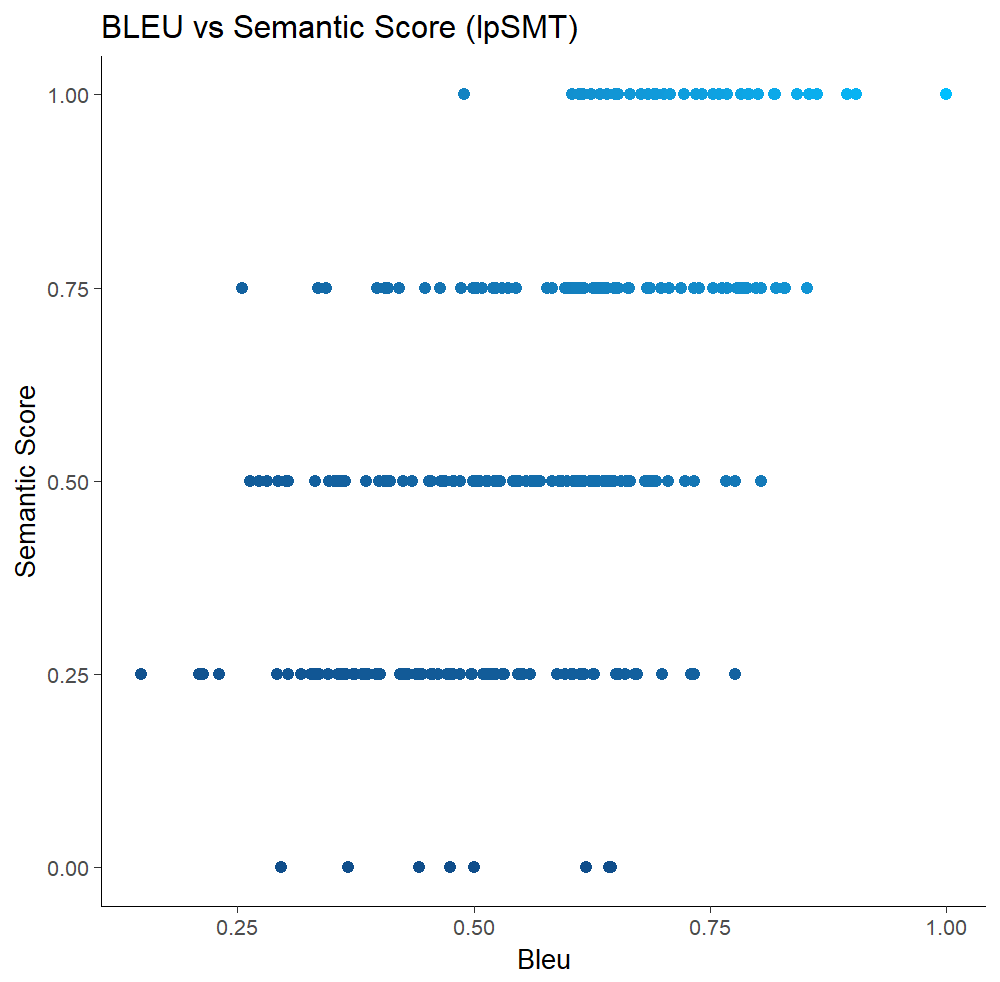
\includegraphics{img/bleuvssemantic_lpSMT.png}
\label{fig:BleuSemlpSMT}
\end{figure}

\begin{figure}
\caption{BLEU vs Semantic (mppSMT)}
\centering
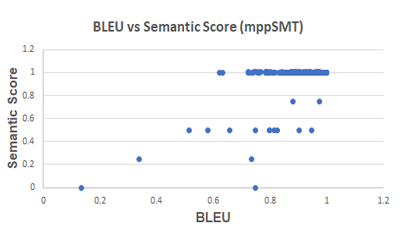
\includegraphics{img/bleuvssemantic_mppSMT.png}
\label{fig:BleuSemMppSMT}
\end{figure}

